\documentclass[12pt,a4paper]{article}

\usepackage[utf8]{inputenc}
\usepackage[T1]{fontenc}
\usepackage{amsmath,amssymb}
\usepackage{graphicx}
\usepackage{booktabs}
\usepackage{natbib}
\usepackage{hyperref}
\usepackage{geometry}
\usepackage{setspace}
\usepackage{caption}
\usepackage{subcaption}
\usepackage{float}
\usepackage{multirow}
\usepackage{xcolor}

\geometry{margin=2.5cm}
\onehalfspacing

\hypersetup{
    colorlinks=true,
    linkcolor=blue!60!black,
    citecolor=blue!60!black,
    urlcolor=blue!60!black
}

\title{\textbf{Spatial Price Indices for Hotel Accommodation in Italy:\\New Evidence from Web-Scraped Data}}

\author{
    Niccolò Salvini\thanks{DEIM, University of Tuscia. E-mail: \texttt{niccolo.salvini@unitus.it}} \and
    Ilaria Benedetti\thanks{Department of Economics, Engineering, Society and Business Organization (DEIm), University of Tuscia. E-mail: \texttt{ilaria.benedetti@unitus.it}} \and
    Tiziana Laureti\thanks{DEIM, University of Tuscia. E-mail: \texttt{laureti@unitus.it}} \and
    Luigi Palumbo\thanks{Banca d'Italia. E-mail: \texttt{luigi.palumbo@bancaditalia.it}}
}

\date{\today}

\begin{document}

\maketitle

\begin{abstract}
Detailed and spatially disaggregated price data for accommodation services are notoriously scarce, limiting the scope of sub-national price comparisons in the tourism sector. This paper addresses this gap by constructing a novel dataset of hotel prices across all Italian provinces through automated web scraping of a major meta-search platform. We adapt the Country Product Dummy (CPD) method---a standard tool for international purchasing power parities---to compute hedonic Spatial Price Indices (SPIs) at the provincial level, controlling for hotel quality, service type, and online reputation. Spatial analysis based on Moran's $I$ statistic and Local Indicators of Spatial Association (LISA) reveals significant positive spatial autocorrelation in hotel prices and identifies well-defined clusters: a high-price belt in the Alpine provinces and persistent low-price zones in the South. The resulting SPIs show that quality-adjusted hotel prices in Bolzano are nearly three times the national average, while several southern provinces lie below 80. These findings demonstrate the potential of web-scraped data for producing timely, granular price statistics for policy and consumer information.

\medskip
\noindent \textbf{Keywords:} Spatial Price Index, web scraping, hotel prices, Country Product Dummy, hedonic regression, spatial autocorrelation, Italy.

\medskip
\noindent \textbf{JEL codes:} C43, C81, L83, R12.
\end{abstract}

%% ============================================================
\section{Introduction}
\label{sec:introduction}
%% ============================================================

Tourism is a major contributor to the Italian economy, accounting for roughly 6.2\% of gross value added---among the highest shares in the European Union \citep{eurostat2023tsa}. The sector's digital transformation has accelerated in recent years, with online booking platforms now mediating a substantial fraction of accommodation transactions. This shift has generated unprecedented volumes of price and availability data in digital form, yet official statistics on accommodation prices remain coarse, typically limited to national or regional averages published with considerable delay.

The lack of spatially granular price data is not merely a statistical inconvenience. For consumers, it means limited transparency about how accommodation costs vary across destinations. For policymakers, it hampers the design of spatially targeted interventions to promote regional competitiveness and manage tourism flows. For researchers, it leaves a conspicuous gap in the empirical landscape: while international price comparisons through Purchasing Power Parities (PPPs) are well established \citep{eurostat_oecd2012}, sub-national spatial price indices for specific service sectors remain rare.

This paper makes three contributions. First, we construct a novel, micro-level dataset of hotel prices covering all 107 Italian provinces through automated web scraping of CozyCozy, a meta-search engine that aggregates listings from major booking platforms including Booking.com, Expedia, and Airbnb. The dataset contains information on nearly 4{,}000 unique hotels, including nightly prices, star ratings, service types, and customer review scores. Second, we adapt the Country Product Dummy (CPD) method---the workhorse model behind Eurostat's international price comparisons \citep{rao2005equivalence}---to the sub-national setting, estimating hedonic Spatial Price Indices (SPIs) that control for observable quality differences across hotels. Third, we complement the index number analysis with exploratory spatial methods, including global and local measures of spatial autocorrelation, to characterize the geography of hotel price differentials in Italy.

Our results reveal marked and spatially structured price disparities. After controlling for hotel category, service type, and online reputation, the province of Bolzano exhibits quality-adjusted prices nearly 2.75 times the national average, followed by Milano and selected provinces in Sardinia and Trentino. At the opposite end, several southern provinces display SPIs well below 100. Local Indicators of Spatial Association (LISA) confirm the presence of statistically significant high--high clusters in the Alpine arc and low--low clusters in parts of the Mezzogiorno.

The paper proceeds as follows. Section~\ref{sec:literature} reviews the relevant literature on spatial price comparisons, the CPD method, and the use of web-scraped data in economic statistics. Section~\ref{sec:data} describes the data source, collection process, and quality control procedures. Section~\ref{sec:methodology} presents the hedonic CPD model and the spatial analysis framework. Section~\ref{sec:results} reports the empirical findings, and Section~\ref{sec:conclusion} discusses implications and avenues for future research.

%% ============================================================
\section{Related Literature}
\label{sec:literature}
%% ============================================================

\subsection{Spatial price comparisons and purchasing power parities}

The measurement of price level differences across geographical areas has a long tradition in economics. At the international level, the International Comparison Program (ICP) and the Eurostat--OECD PPP Programme produce regular estimates of purchasing power parities for broad expenditure aggregates \citep{eurostat_oecd2012, worldbank2020icp}. These comparisons rely on structured price surveys and well-established index number methods, among which the Country Product Dummy (CPD) regression plays a central role.

The CPD method, introduced by \citet{summers1973} and refined by \citet{rao2005equivalence}, estimates price level differences across countries (or regions) by regressing the logarithm of observed prices on a set of area and product dummy variables. The exponentials of the area coefficients yield multilateral price indices that satisfy transitivity and are robust to differences in product availability across locations. The method extends naturally to hedonic specifications when product characteristics are continuous rather than categorical \citep{silver2009hedonic, diewert2010hedonic}.

Sub-national applications of the CPD framework are less common but have gained momentum. \citet{breton2015spatial} estimated spatial price indices across French departments; \citet{majari2017spatial} applied the method to Iranian provinces. For Italy, sub-national spatial price comparisons have been developed along several lines. \citet{biggeri2017provincial} used small area estimation to produce provincial-level household consumption estimates in real terms, applying PPPs derived from the CPD method to deflate nominal expenditure. \citet{laureti2020spatial} computed food price indices across Italian regions using scanner data. More recently, \citet{biggeri2022housing} constructed spatial price indices for housing rents at the regional level, adapting the hedonic CPD to accommodate the pronounced heterogeneity of rental markets. \citet{laureti2024food} extended the framework to a spatial-temporal setting, estimating food affordability indices across Italian regions using web-scraped price data within a Time-interaction-Region Product Dummy (TiRPD) model. Despite this progress, spatially disaggregated price indices for accommodation services remain virtually absent, primarily because of data limitations.

\subsection{Hedonic pricing of hotel accommodation}

Hedonic price models decompose observed prices into implicit valuations of product characteristics \citep{rosen1974hedonic}. In the hotel industry, a large literature has identified the key determinants of room prices, including star rating, location, amenities, seasonality, and---increasingly---online reputation \citep{zhang2011determinants, espinet2003effect}.

Recent studies have exploited data from online travel agencies (OTAs) and review platforms to estimate hedonic price functions at fine spatial and temporal resolution. \citet{kim2021hedonic} showed that customer ratings and review volume significantly affect willingness to pay, even after controlling for objective quality indicators. \citet{choi2022hedonic} developed hedonic indices for the Korean hotel market using scraped data and documented substantial price heterogeneity across regions. \citet{li2023bigdata} demonstrated the feasibility of large-scale hedonic analysis using big data techniques. Our work differs from this literature in that we do not aim to explain price variation per se, but rather to purge it of quality differences in order to isolate the pure spatial component---the Spatial Price Index.

\subsection{Web scraping as a data source for economic statistics}

The use of automatically collected online data for price measurement has been pioneered by the Billion Prices Project \citep{cavallo2016billion}, which demonstrated that daily scraped retail prices closely track official CPI movements with much higher frequency. Since then, national statistical offices and international organizations have progressively integrated web-scraped data into their production processes \citep{eurostat2020webscraping, tenBosch2020webscraping}.

In the tourism domain, web scraping has been used to study short-term rental markets \citep{gibbs2018pricing}, hotel pricing strategies \citep{abrate2012dynamic}, and market structure on OTA platforms \citep{hunold2018resale}. A related methodological challenge concerns the evaluation of \textit{coverage}---the extent to which scraped prices adequately represent the target market. \citet{palumbo2023coverage} proposed a geostatistical fuzzy index that measures the geographical and population coverage of web-scraped grocery prices in Italy, offering a principled framework for assessing representativeness that extends naturally to other domains, including accommodation. Despite these advances, the use of scraped data for constructing spatial price indices in the accommodation sector---as opposed to analysing pricing behaviour---remains largely unexplored. This paper bridges the gap between the web scraping literature and the spatial price comparison literature by showing how scraped hotel prices, combined with the CPD framework, can produce informative sub-national price level indicators.

%% ============================================================
\section{Data}
\label{sec:data}
%% ============================================================

\subsection{Data source}

The price data used in this study are collected from CozyCozy (\url{https://www.cozycozy.com}), a meta-search engine for accommodation that aggregates listings from over 100 booking platforms, including Booking.com, Expedia, Hotels.com, Trip.com, Airbnb, and Vrbo. Unlike single-platform datasets, CozyCozy offers a consolidated view of the accommodation market, reducing the selection bias inherent in relying on any individual online travel agency.

For each listing, the platform reports the property name, geographical coordinates, nightly price, star rating, type of service (room only, bed and breakfast, half board, full board), room type, customer rating score, number of reviews, available providers and their respective prices, and a range of amenity indicators.

\subsection{Data collection infrastructure}

Collecting price data at the scale and frequency required for spatial comparisons across all Italian provinces is a non-trivial engineering task. The DataLab at the University of Tuscia has developed a fully automated data collection system---designed, deployed, and maintained in-house---that operates on a daily schedule without manual intervention.

The infrastructure rests on three components. First, the \textit{scraping engine} combines two complementary extraction strategies: (i) reverse engineering of the platform's internal API endpoints, which allows direct retrieval of structured JSON responses when available, and (ii) browser-based automation via Selenium for dynamic content that is only rendered client-side. To achieve the throughput needed to cover 107 provinces within a reasonable time window, the system uses Selenium Grid to distribute scraping tasks across multiple containerised browser instances running in parallel. Second, a \textit{traffic management layer} based on GlueTun routes requests through rotating proxies, ensuring IP anonymisation and mitigating the risk of access restrictions. Third, all collected data flow into a centralised PostgreSQL database where they are time-stamped, deduplicated, and made available for downstream statistical analysis.

The full pipeline executes daily at 12:00 CET, issuing location-specific search queries for a standardised booking profile (one guest, one room, one night) across all 107 Italian provinces. Each complete cycle takes approximately three hours. The modular, containerised architecture (orchestrated via Docker Compose) allows rapid adaptation when the target platform modifies its page structure or access policies---a frequent occurrence in web scraping projects.

While the system is designed for continuous daily collection, the analysis in this paper focuses on a cross-sectional snapshot collected on 10 December 2024. We restrict the sample to hotel accommodation (excluding vacation rentals, hostels, and other non-hotel property types) identified by their star classification (1 to 5 stars). Properties without a valid star rating or with ambiguous categorisation are excluded.

\subsection{Data processing and quality control}

Raw scraped data require careful processing before they can be used for price comparisons. We implement a multi-stage cleaning procedure.

\paragraph{Spatial deduplication.}
The same hotel may appear multiple times in the dataset because different booking platforms list it independently, sometimes with slightly different names or coordinates. To resolve this, we apply DBSCAN clustering \citep{ester1996density} with a 50-metre radius to group listings that are spatially proximate. Within each spatial cluster, we apply fuzzy string matching on hotel names using the Jaro--Winkler distance \citep{winkler1990string}, with a threshold of 0.2. Listings identified as duplicates are reconciled as follows: exact duplicates (same hotel, same offer, same price) are collapsed to a single observation; listings with the same offer type but different prices are resolved by retaining the lowest price; and listings with genuinely different offers (e.g., room only vs.\ bed and breakfast) are kept as separate observations.

\paragraph{Outlier removal.}
We remove extreme price observations following industry-specific heuristics. Prices exceeding \texteuro25{,}000 per night are dropped unconditionally (these typically reflect data entry errors or luxury villa listings miscategorized as hotels). For lower-star categories (1--3 stars), an upper threshold of \texteuro3{,}000 is applied, while suite offers above \texteuro5{,}000 are also excluded. The placeholder value of \texteuro1{,}000{,}000 (used by the platform for unavailable listings) is removed.

\paragraph{Final dataset.}
After cleaning, the dataset contains 3{,}958 unique hotel--offer observations across 1{,}285 cities and all 107 Italian provinces. Table~\ref{tab:summary} presents summary statistics by hotel category.

\begin{table}[H]
\centering
\caption{Summary statistics by hotel category.}
\label{tab:summary}
\begin{tabular}{lccccc}
\toprule
\textbf{Category} & \textbf{$N$} & \textbf{Mean price (\texteuro)} & \textbf{Median price (\texteuro)} & \textbf{Mean rating} & \textbf{\% Breakfast} \\
\midrule
Hotel 1* & 108  & 71.19  & 67.15  & 77.67 & 10.2 \\
Hotel 2* & 351  & 78.42  & 70.00  & 79.50 & 16.0 \\
Hotel 3* & 1{,}965 & 91.69  & 80.00  & 81.92 & 20.9 \\
Hotel 4* & 1{,}417 & 120.68 & 104.00 & 82.85 & 26.7 \\
Hotel 5* & 117  & 248.32 & 198.00 & 86.14 & 35.5 \\
\midrule
Total    & 3{,}958 & & & & \\
\bottomrule
\end{tabular}
\end{table}

Three-star hotels constitute nearly half the sample, reflecting the structure of the Italian hotel market. Mean and median prices increase monotonically with star rating, as expected, though the distributions are right-skewed within each category. Higher-rated hotels also tend to have better customer ratings and a higher incidence of breakfast inclusion in the base price.

\subsection{Coverage assessment}

To evaluate the representativeness of the scraped sample, we compare the number of hotels in our dataset with ISTAT official counts of accommodation establishments by province and star category. While exact coverage rates vary across provinces and categories, the dataset captures a substantial share of the hotel population, particularly for 3- and 4-star hotels in major tourist provinces. Provinces with lower tourism intensity tend to have lower coverage, which we address in the estimation by restricting the SPI analysis to provinces with sufficient observations.

%% ============================================================
\section{Methodology}
\label{sec:methodology}
%% ============================================================

\subsection{The hedonic CPD model for spatial price indices}

We adapt the Country Product Dummy (CPD) regression to the sub-national setting. In the standard international application, the CPD model regresses the logarithm of prices on country and product dummies \citep{rao2005equivalence}. The approach has been applied within Italy to food and housing \citep{laureti2020spatial, biggeri2022housing}; here, we extend it to accommodation services, where provinces replace countries and hotel characteristics replace product categories.

Let $p_{ij}$ denote the price of hotel $i$ located in province $j$. The hedonic CPD model is specified as:

\begin{equation}
\label{eq:cpd}
\ln p_{ij} = \sum_{j=1}^{J} \beta_j \, D_j^{\text{prov}} + \sum_{s=1}^{S} \gamma_s \, D_s^{\text{star}} + \sum_{k=1}^{K} \delta_k \, D_k^{\text{offer}} + \theta_1 \, \textit{RatingScore}_i + \theta_2 \, \textit{RatingCount}_i + \varepsilon_{ij}
\end{equation}

\noindent where $D_j^{\text{prov}}$ are province dummies, $D_s^{\text{star}}$ are star-category dummies, $D_k^{\text{offer}}$ are dummies for the type of service (room only, bed and breakfast, half board, full board), $\textit{RatingScore}_i$ is the customer rating on a 0--100 scale, and $\textit{RatingCount}_i$ is the number of reviews.

The province dummies are coded using a sum-to-zero constraint:
\begin{equation}
\sum_{j=1}^{J} \beta_j = 0
\end{equation}
This ensures that the reference level is the unweighted mean across all provinces, rather than a single arbitrarily chosen province. The \textit{Spatial Price Index} (SPI) for province $j$ is then computed as:
\begin{equation}
\label{eq:spi}
\text{SPI}_j = \exp(\hat{\beta}_j) \times 100
\end{equation}
A value of $\text{SPI}_j > 100$ indicates that quality-adjusted hotel prices in province $j$ exceed the national average, while $\text{SPI}_j < 100$ indicates the opposite. By construction, the unweighted mean of the SPI across provinces equals 100.

The inclusion of hedonic controls---star rating, service type, and reputation---serves a dual purpose. First, it purges observed price differences of quality variation, so that the SPI captures the ``pure'' spatial price differential: how much more or less one pays for a comparable hotel room in province $j$ relative to the national average. Second, it reduces omitted variable bias that would arise if, for example, high-price provinces also have a disproportionate share of luxury hotels.

\subsection{Alternative specifications}

We estimate three variants of the CPD model to assess robustness:
\begin{enumerate}
    \item[(i)] \textbf{Pooled model}: All star categories pooled, with star dummies as controls (Equation~\ref{eq:cpd}).
    \item[(ii)] \textbf{Category-specific model}: Restricted to 3-star hotels only (the modal category), with no star dummies but retaining the service and reputation controls.
    \item[(iii)] \textbf{Binary stratification}: Hotels grouped into two classes (1--3 stars and 4--5 stars), with a binary quality indicator.
\end{enumerate}
The category-specific model has the advantage of comparing strictly homogeneous products---akin to comparing prices of the same good across countries---but at the cost of a reduced sample. The pooled model leverages the full dataset and relies on the star dummies to capture inter-category price differences. We report the category-specific 3-star results as our baseline and use the other specifications for robustness.

\subsection{Spatial analysis}
\label{sec:spatial_methods}

To characterize the spatial structure of hotel prices, we employ two complementary approaches.

\paragraph{Global spatial autocorrelation.}
We compute Moran's $I$ statistic \citep{moran1950notes} on provincial mean prices:
\begin{equation}
I = \frac{N}{\sum_{j}\sum_{k} w_{jk}} \cdot \frac{\sum_{j}\sum_{k} w_{jk}(y_j - \bar{y})(y_k - \bar{y})}{\sum_{j}(y_j - \bar{y})^2}
\end{equation}
where $y_j$ is the mean hotel price in province $j$, $w_{jk}$ is the spatial weight linking provinces $j$ and $k$ (we use first-order Queen contiguity), and $N$ is the number of provinces. A significantly positive $I$ indicates that nearby provinces tend to have similar prices (positive spatial autocorrelation).

At the individual hotel level, we also compute Moran's $I$ using a $k$-nearest-neighbour weight matrix ($k=5$) based on hotel coordinates, to assess micro-level spatial dependence.

\paragraph{Local indicators of spatial association.}
To identify localized price clusters, we compute Local Moran's $I_j$ statistics \citep{anselin1995local}:
\begin{equation}
I_j = \frac{(y_j - \bar{y})}{\sigma^2} \sum_{k} w_{jk}(y_k - \bar{y})
\end{equation}
with inference based on a conditional permutation approach (999 permutations). The LISA analysis classifies each province into one of four quadrants: High--High (expensive provinces surrounded by expensive neighbours), Low--Low (cheap provinces surrounded by cheap neighbours), High--Low, and Low--High. Provinces whose local Moran statistic is significant at the 5\% level are mapped to identify spatial clusters and outliers.

%% ============================================================
\section{Results}
\label{sec:results}
%% ============================================================

\subsection{Price distributions}

Figure~\ref{fig:price_dist} displays the distribution of log prices by hotel category. Within each star class, the distributions are approximately log-normal, with right tails that are more pronounced for higher categories. The interquartile range widens substantially from 1-star to 5-star hotels, reflecting the greater heterogeneity of the luxury segment. These distributional features motivate the use of a log-linear model.

\begin{figure}[H]
    \centering
    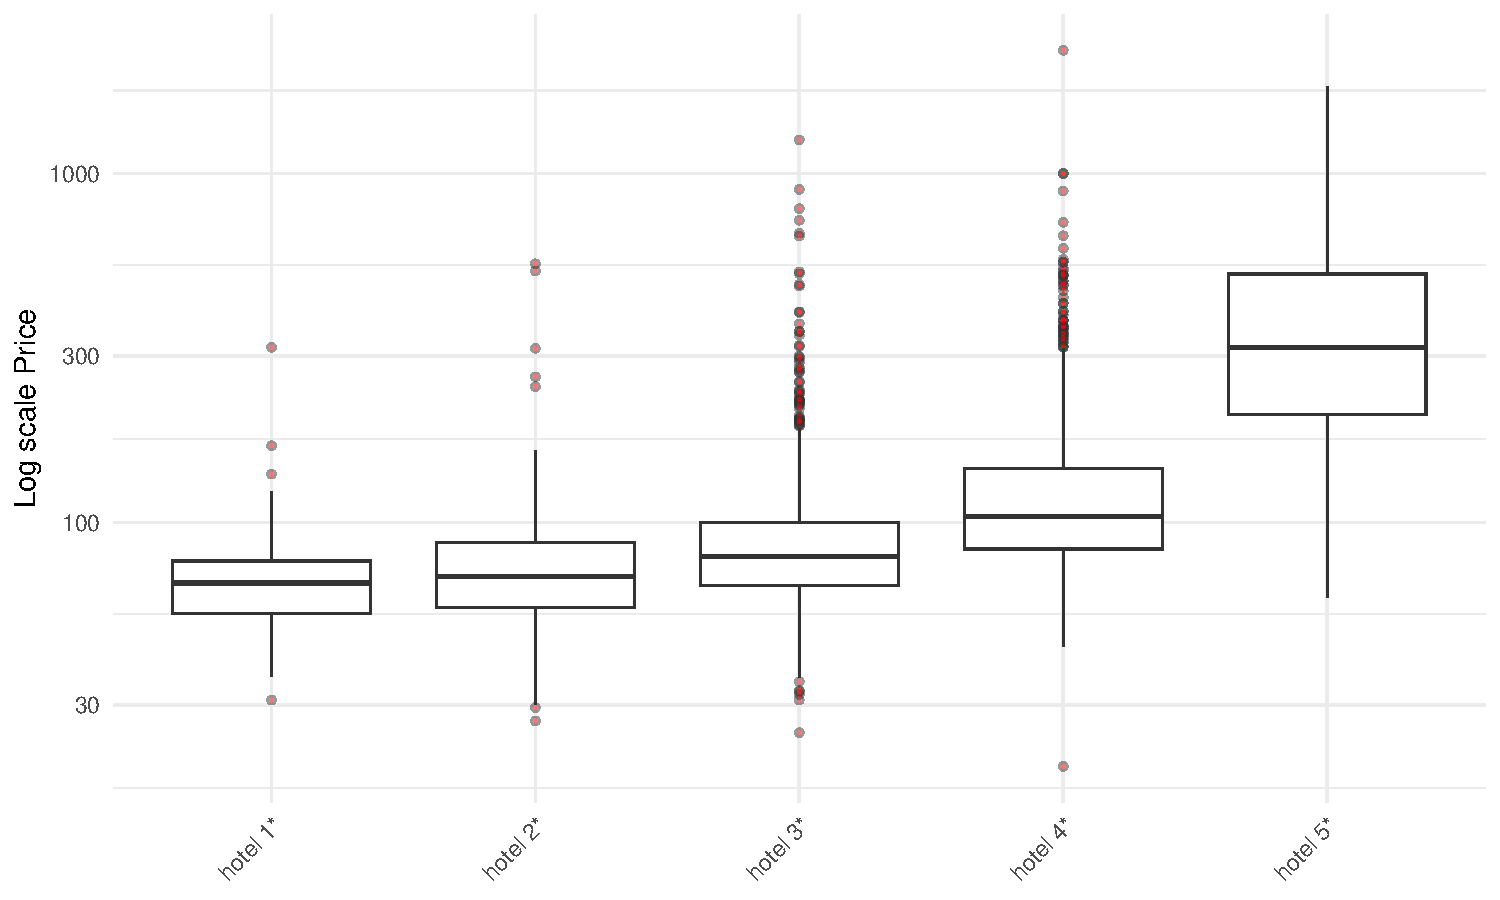
\includegraphics[width=\textwidth]{../images/hotel_price_distribution.pdf}
    \caption{Hotel price distribution by star category (log scale).}
    \label{fig:price_dist}
\end{figure}

The gap between mean and median within each category (Table~\ref{tab:summary}) signals positive skewness, driven by a tail of high-priced listings. This skewness is more severe for upper categories: among 5-star hotels, the mean exceeds the median by over \texteuro50, indicating the presence of a luxury segment with prices far above the category norm. Within each star class, exploratory GAM regressions of price on the customer rating score reveal a non-linear relationship: prices rise steeply for ratings above approximately 80, while the association is flat and noisy at lower levels, suggesting that online reputation acts as a price premium only above a perceived quality threshold.

\subsection{Spatial autocorrelation}

Figure~\ref{fig:moran} presents the Moran scatterplot for individual hotel prices, using a $k$-nearest-neighbour weight matrix with $k=5$. The significantly positive slope confirms the presence of global spatial autocorrelation: hotels located near each other tend to charge similar prices, even across different star categories. Several outliers are visible in the upper-right quadrant (high-price hotels in high-price neighbourhoods), often corresponding to luxury properties in established tourist destinations.

\begin{figure}[H]
    \centering
    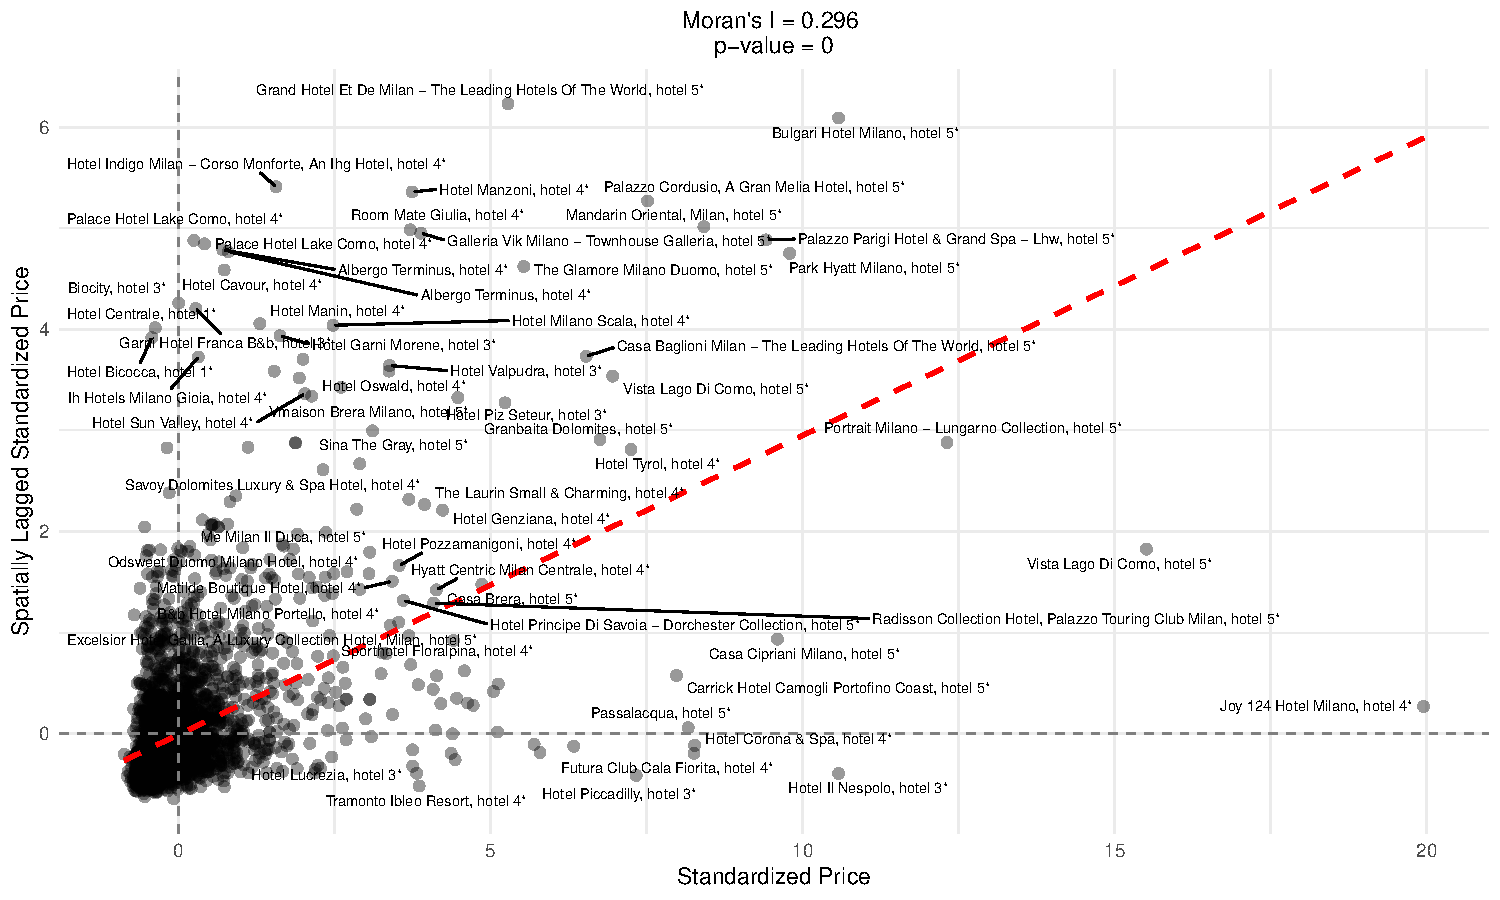
\includegraphics[width=0.85\textwidth]{../images/moran_plot.pdf}
    \caption{Moran scatterplot of individual hotel prices ($k$=5 nearest neighbours).}
    \label{fig:moran}
\end{figure}

\subsection{Local spatial clusters: LISA analysis}

The LISA map in Figure~\ref{fig:lisa} identifies statistically significant local price clusters at the provincial level. Two patterns dominate.

First, a contiguous cluster of High--High provinces extends across the Alpine arc, centred on Bolzano and Trento and reaching into Sondrio and neighbouring areas. These provinces host major ski resorts and are characterised by a combination of constrained accommodation supply, high international demand, and a concentration of upper-category hotels. Crucially, the December collection date captures the beginning of the winter ski season, which inflates prices in Alpine destinations well above their annual average. The prominence of this cluster should therefore be interpreted with caution: the same analysis conducted in, say, July would likely attenuate the Alpine premium and strengthen the relative position of coastal and island provinces that are in low season in December.

Second, a band of Low--Low provinces spans parts of southern Italy, including inland Calabria, Basilicata, and Sicily. These areas are characterised by lower tourism intensity, weaker transport connectivity, and a predominance of lower-category hotels. However, the winter snapshot also penalises these provinces: many southern coastal destinations experience their demand peak in summer, and their December prices reflect off-season conditions. The apparent north--south gradient is therefore a composite of structural price differences and seasonal timing, and disentangling the two requires repeated observations across seasons.

Spatial outliers (High--Low and Low--High) are less frequent but informative. Isolated High--Low provinces correspond to cities with demand drivers that are relatively season-invariant---business travel, pilgrimage, or cultural tourism---surrounded by lower-price hinterlands.

\begin{figure}[H]
    \centering
    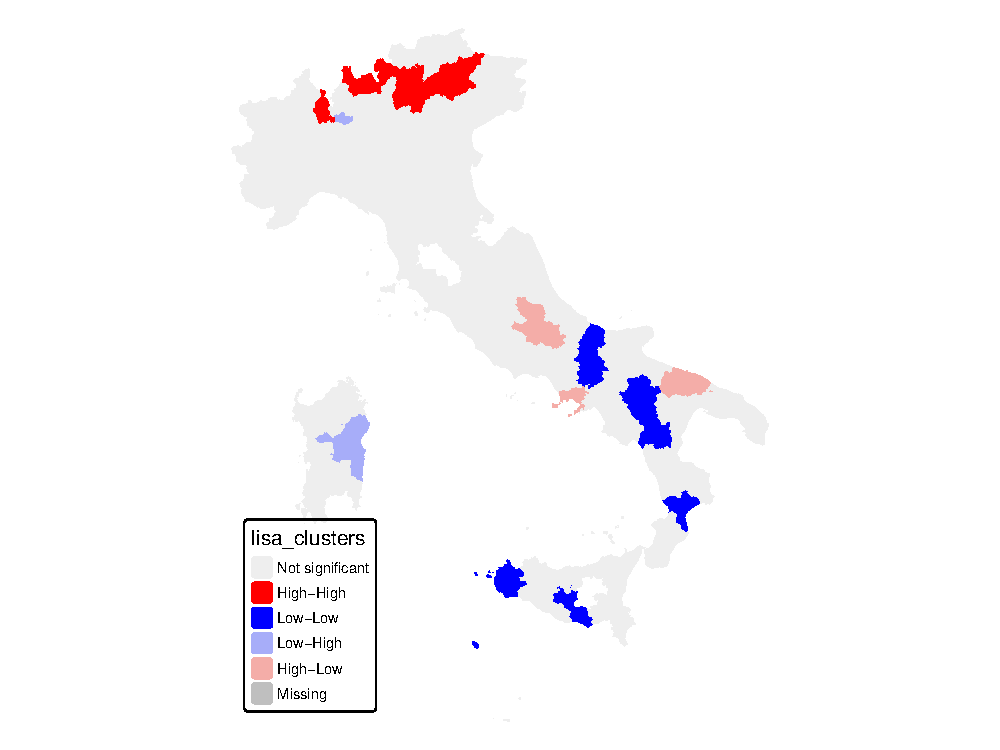
\includegraphics[width=0.85\textwidth]{../images/lisa_map.pdf}
    \caption{LISA cluster map of mean hotel prices at the provincial level.}
    \label{fig:lisa}
\end{figure}

\subsection{Spatial Price Index results}

Table~\ref{tab:spi} reports the estimated SPIs for the ten most expensive provinces, based on the category-specific model for 3-star hotels with hedonic controls (offer type, rating score, review count). The province of Bolzano stands out with an SPI of 275, meaning that a comparable 3-star hotel room costs 2.75 times the national average. This extreme value reflects both a structural premium---Bolzano has a small, high-quality hotel stock serving strong international demand---and a seasonal component: December marks the height of the ski season in South Tyrol. A summer snapshot would likely yield a lower, though still above-average, SPI for Bolzano. Milano follows at 144, driven by business travel and event-related demand that is less seasonally dependent. Two Sardinian provinces (Oristano and Sassari) rank third and fourth; their high SPIs, combined with large standard errors ($t$-statistics of 1.99 and 2.53), suggest that these estimates are based on a relatively thin sample and should be interpreted with particular caution.

\begin{table}[H]
\centering
\caption{Spatial Price Index: top 10 provinces (national average = 100).}
\label{tab:spi}
\begin{tabular}{lcccr}
\toprule
\textbf{Province} & \textbf{$\hat{\beta}_j$} & \textbf{Std.\ error} & \textbf{$t$-stat} & \textbf{SPI} \\
\midrule
Bolzano  & 1.010 & 0.084 & 12.00 & 275 \\
Milano   & 0.363 & 0.032 & 11.20 & 144 \\
Oristano & 0.306 & 0.154 &  1.99 & 136 \\
Sassari  & 0.287 & 0.113 &  2.53 & 133 \\
Trento   & 0.252 & 0.031 &  8.05 & 129 \\
Sondrio  & 0.212 & 0.050 &  4.25 & 124 \\
Como     & 0.199 & 0.044 &  4.56 & 122 \\
Lecce    & 0.199 & 0.134 &  1.48 & 122 \\
Genova   & 0.196 & 0.122 &  1.61 & 122 \\
Lucca    & 0.190 & 0.051 &  3.70 & 121 \\
\bottomrule
\end{tabular}
\end{table}

The geographic distribution of the SPI is mapped in Figure~\ref{fig:spi_map}. The map reinforces the north--south gradient documented in the LISA analysis but adds nuance. Several central Italian provinces---Lucca, Como, and Lecce---exhibit above-average SPIs, consistent with the presence of high-value cultural and lakeside tourism. The eastern Adriatic coast, which hosts large volumes of mass beach tourism, shows relatively moderate price levels, suggesting that high demand does not necessarily translate into high prices when accommodation supply is abundant.

\begin{figure}[H]
    \centering
    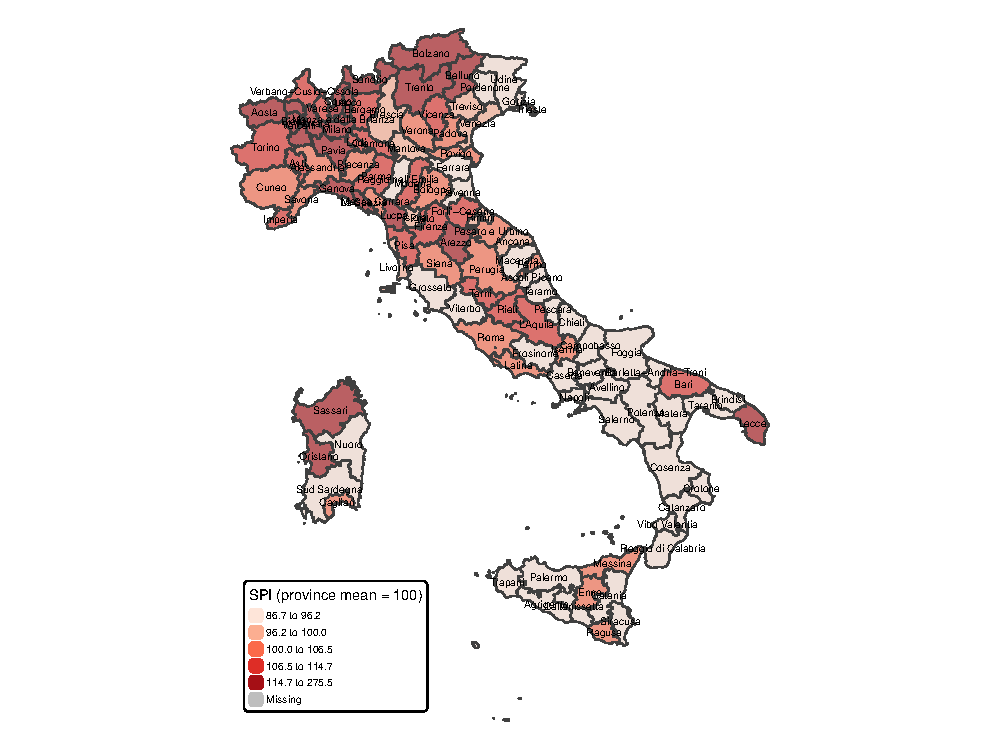
\includegraphics[width=0.85\textwidth]{../images/spi_map.pdf}
    \caption{Spatial Price Index by province (national average = 100).}
    \label{fig:spi_map}
\end{figure}

A number of caveats apply to the interpretation of these results. First, provinces with few 3-star hotel observations (Oristano, Lecce, Genova) yield imprecise estimates, as reflected in their large standard errors and low $t$-statistics. Their ranking should be treated as indicative rather than definitive. Second, the single-date extraction means that the SPI captures a winter pricing equilibrium: provinces whose tourism is predominantly summer-oriented (e.g., much of the southern coastline and the islands) are observed at their off-season prices, while Alpine and urban destinations are at or near their seasonal peak. The resulting north--south price gradient therefore conflates structural spatial differentials with seasonal timing. Disentangling the two would require repeated cross-sections spanning at least a full calendar year, which the data infrastructure described in Section~\ref{sec:data} is designed to support in future work. Third, the coverage of the scraped dataset, while broad, is not uniform: small, independent hotels that do not list on major online platforms are underrepresented, potentially biasing the SPI towards the segment of the market that is most visible online. As \citet{palumbo2023coverage} have argued in the context of grocery prices, a formal coverage assessment is essential when web-scraped data are used for price index construction.

Notwithstanding these limitations, the core findings---the Alpine premium, the Milano effect, and the southern discount---are robust across the alternative specifications described in Section~\ref{sec:methodology}. In the pooled model with all star categories, the rank ordering of provinces is preserved, with Bolzano, Milano, and Trento consistently among the most expensive.


%% ============================================================
\section{Discussion and Conclusions}
\label{sec:conclusion}
%% ============================================================

This paper demonstrates that web-scraped data from online accommodation platforms can be used to construct meaningful sub-national Spatial Price Indices for hotel services. By combining a rich micro-level dataset with the CPD hedonic framework---adapted from the international PPP literature---we provide the first systematic comparison of quality-adjusted hotel prices across all Italian provinces.

Three main findings emerge. First, spatial price differentials in the Italian hotel market are large: the ratio between the most expensive province (Bolzano, SPI $= 275$) and the cheapest is on the order of three to one, even after controlling for hotel quality and service type. Second, these differentials are not randomly distributed but exhibit strong spatial structure, with high-price clusters in the Alps and the northern lakes and low-price clusters in parts of the South. Third, online reputation---measured by customer ratings and review counts---has a significant and non-linear effect on prices, reinforcing the importance of hedonic controls in spatial price comparisons.

Several implications follow. From a \textit{statistical} perspective, the results show that web-scraped accommodation data are a viable complement to traditional price collection methods. The CPD framework is well suited to handle the high-dimensional, unbalanced nature of scraped datasets, and the resulting indices are interpretable within the established PPP framework. From a \textit{policy} perspective, the SPIs provide actionable information for tourism planning. The identification of persistent high- and low-price zones can inform strategies for spatial redistribution of tourism flows, pricing regulation, and investment in underserved areas. From a \textit{consumer} perspective, quality-adjusted price comparisons enhance transparency and help travellers make informed choices beyond headline prices.

These results should be read against the limitations that the current dataset imposes. The most consequential is the reliance on a single cross-section collected in December. Hotel prices in Italy are highly seasonal: the winter period favours Alpine and urban destinations while depressing prices in southern coastal and island areas. The SPIs presented here therefore capture a winter pricing equilibrium that is not representative of the annual average. The magnitude of the Bolzano premium (SPI $= 275$) is almost certainly inflated by ski-season demand, and the relative cheapness of provinces like Crotone or Agrigento reflects off-season pricing rather than---or in addition to---structural cost differences. Without repeated observations across the calendar year, separating the seasonal component from the permanent spatial differential is not possible with the present data.

A second limitation concerns data coverage. The scraped dataset, while geographically comprehensive, reflects the segment of the hotel market that is listed on major online platforms. Small, family-run hotels---particularly common in the South and in inland areas---may be underrepresented. To the extent that such establishments charge lower prices, the SPIs for less digitised provinces may be biased upward. Formal evaluation of scraping coverage, along the lines proposed by \citet{palumbo2023coverage} for grocery prices, is a priority for future work.

Third, the hedonic specification, while parsimonious, does not capture all observable quality dimensions. Amenities (pool, spa, parking), location within the city (distance to the centre or to transport hubs), and room-level characteristics are available in the raw scraped data and could be incorporated in richer specifications.

These limitations also define the natural extensions of this work. The daily collection infrastructure described in Section~\ref{sec:data} is designed to accumulate a longitudinal dataset that will support the estimation of spatial-temporal price indices, following the TiRPD approach of \citet{laureti2024food}, thereby disentangling seasonal from structural price variation. Incorporating spatial econometric models---spatial lag or spatial error specifications---directly into the CPD estimation would allow the SPI itself to account for spatial spillovers between neighbouring provinces. Finally, the methodology is portable: the same framework can be applied to other accommodation types (B\&Bs, vacation rentals) and to other countries where meta-search platforms operate, opening the way for cross-national spatial price comparisons of tourism services.

\paragraph{Acknowledgements.}
This research was supported by the PRIN programme of the Italian Ministry of University and Research (MUR), grant year 2022. We thank Federico Crescenzi and Luigi Palumbo for helpful discussions.

%% ============================================================
%% REFERENCES
%% ============================================================
\newpage
\begin{thebibliography}{99}

\bibitem[Abrate et al.(2012)]{abrate2012dynamic}
Abrate, G., Fraquelli, G., and Viglia, G. (2012).
Dynamic pricing strategies: Evidence from European hotels.
\textit{International Journal of Hospitality Management}, 31(1):160--168.

\bibitem[Anselin(1995)]{anselin1995local}
Anselin, L. (1995).
Local Indicators of Spatial Association---LISA.
\textit{Geographical Analysis}, 27(2):93--115.

\bibitem[Antolini et al.(2024)]{antolini2024integrating}
Antolini, F., Terraglia, I., and Cesarini, S. (2024).
Integrating multiple data sources to measure sustainable tourism in Italian regions.
\textit{Socio-Economic Planning Sciences}, 93:101959.

\bibitem[Arbia et al.(2024)]{arbia2024unconventional}
Arbia, G., et al. (2024).
Unconventional data sources and big data analytics for innovation in economic statistics.
Working paper.

\bibitem[Biggeri et al.(2017)]{biggeri2017provincial}
Biggeri, L., Laureti, T., and Polidoro, F. (2017).
Estimates of household consumption expenditure at provincial level in Italy by using small area estimation methods: ``Real'' comparisons using purchasing power parities.
\textit{Social Indicators Research}, 131(1):215--243.

\bibitem[Biggeri and Laureti(2022)]{biggeri2022housing}
Biggeri, L. and Laureti, T. (2022).
Sub-national spatial price indexes for housing: Methodological issues and computation for Italy.
\textit{Journal of Official Statistics}, 38(1):57--82.

\bibitem[Breton and Eyraud(2015)]{breton2015spatial}
Breton, R. and Eyraud, L. (2015).
Spatial price comparisons across French departments.
\textit{Economics and Statistics}, 477:15--39.

\bibitem[Cavallo and Rigobon(2016)]{cavallo2016billion}
Cavallo, A. and Rigobon, R. (2016).
The Billion Prices Project: Using online prices for measurement and research.
\textit{Journal of Economic Perspectives}, 30(2):151--178.

\bibitem[Choi et al.(2022)]{choi2022hedonic}
Choi, Y., Kim, J., and Lee, C. (2022).
Hedonic pricing of hotel attributes: A big data approach.
\textit{Tourism Management}, 90:104480.

\bibitem[Diewert(2010)]{diewert2010hedonic}
Diewert, W.E. (2010).
New methodological developments for the International Comparison Program.
\textit{Review of Income and Wealth}, 56(S1):S218--S232.

\bibitem[Espinet et al.(2003)]{espinet2003effect}
Espinet, J.M., Saez, M., Coenders, G., and Fluvi\`a, M. (2003).
Effect on prices of the attributes of holiday hotels: A hedonic prices approach.
\textit{Tourism Economics}, 9(2):165--177.

\bibitem[Ester et al.(1996)]{ester1996density}
Ester, M., Kriegel, H.-P., Sander, J., and Xu, X. (1996).
A density-based algorithm for discovering clusters in large spatial databases with noise.
In \textit{Proceedings of KDD-96}, pp.\ 226--231.

\bibitem[Eurostat(2020)]{eurostat2020webscraping}
Eurostat (2020).
\textit{Web Scraping for Official Statistics}.
Eurostat Methodological Working Paper.

\bibitem[Eurostat(2023)]{eurostat2023tsa}
Eurostat (2023).
\textit{Tourism Satellite Accounts in Europe---2023 Edition}.
Publications Office of the European Union.

\bibitem[Eurostat--OECD(2012)]{eurostat_oecd2012}
Eurostat--OECD (2012).
\textit{Eurostat--OECD Methodological Manual on Purchasing Power Parities}.
Publications Office of the European Union.

\bibitem[Gibbs et al.(2018)]{gibbs2018pricing}
Gibbs, C., Guttentag, D., Gretzel, U., Morton, J., and Goodwill, A. (2018).
Pricing in the sharing economy: A hedonic pricing model applied to Airbnb listings.
\textit{Journal of Travel \& Tourism Marketing}, 35(1):46--56.

\bibitem[Hunold et al.(2018)]{hunold2018resale}
Hunold, M., Kesler, R., Laitenberger, U., and Schlütter, F. (2018).
Evaluation of best price clauses in online hotel bookings.
\textit{International Journal of Industrial Organization}, 61:542--571.

\bibitem[Kim et al.(2021)]{kim2021hedonic}
Kim, D., Hong, S., and Park, B. (2021).
The effects of online reviews on hotel pricing: A hedonic approach.
\textit{International Journal of Hospitality Management}, 95:102885.

\bibitem[Laureti and Ferrara(2020)]{laureti2020spatial}
Laureti, T. and Ferrara, C. (2020).
Spatial price indices for Italian food consumption.
\textit{Social Indicators Research}, 148:541--560.

\bibitem[Laureti et al.(2024)]{laureti2024food}
Laureti, T., Benedetti, I., Palumbo, L., and Crescenzi, F. (2024).
Assessing food affordability in Italy: A spatial-temporal analysis using web-scraped data.
SSRN Working Paper No.\ 4759493.

\bibitem[Li et al.(2023)]{li2023bigdata}
Li, H., Ye, Q., and Law, R. (2023).
Big data and hedonic pricing: Best practices for hotel price analysis.
\textit{Annals of Tourism Research}, 98:103512.

\bibitem[Majari and Hajargasht(2017)]{majari2017spatial}
Majari, J. and Hajargasht, G. (2017).
Sub-national purchasing power parities for Iran.
\textit{Empirical Economics}, 52:1077--1099.

\bibitem[Palumbo et al.(2023)]{palumbo2023coverage}
Palumbo, L., Guillen, M., Laureti, T., and Benedetti, I. (2023).
A geostatistical fuzzy index to measure geographical and population coverage of consumer prices collection: The case of groceries webscraping in Italy.
SSRN Working Paper No.\ 4279435.

\bibitem[Moran(1950)]{moran1950notes}
Moran, P.A.P. (1950).
Notes on continuous stochastic phenomena.
\textit{Biometrika}, 37(1/2):17--23.

\bibitem[Rao(2005)]{rao2005equivalence}
Rao, D.S.P. (2005).
On the equivalence of the weighted country-product-dummy (CPD) method and the Rao-system for multilateral price comparisons.
\textit{Review of Income and Wealth}, 51(4):571--580.

\bibitem[Rosen(1974)]{rosen1974hedonic}
Rosen, S. (1974).
Hedonic prices and implicit markets: Product differentiation in pure competition.
\textit{Journal of Political Economy}, 82(1):34--55.

\bibitem[Silver(2009)]{silver2009hedonic}
Silver, M. (2009).
Do unit value export, import, and terms-of-trade indices misrepresent price indices?
\textit{IMF Staff Papers}, 56(2):297--322.

\bibitem[Summers(1973)]{summers1973}
Summers, R. (1973).
International price comparisons based upon incomplete data.
\textit{Review of Income and Wealth}, 19(1):1--16.

\bibitem[ten Bosch et al.(2020)]{tenBosch2020webscraping}
ten Bosch, O., Windmeijer, D., van de Ven, A., and Buiten, G. (2020).
Web scraping meets survey design: Combining forces.
\textit{Big Data Meets Survey Science}, Wiley, pp.\ 147--172.

\bibitem[World Bank(2020)]{worldbank2020icp}
World Bank (2020).
\textit{Purchasing Power Parities and the Size of World Economies: Results from the 2017 International Comparison Program}.
World Bank, Washington, DC.

\bibitem[Zhang et al.(2011)]{zhang2011determinants}
Zhang, Z., Ye, Q., and Law, R. (2011).
Determinants of hotel room price: An exploration of travelers' hierarchy of accommodation needs.
\textit{International Journal of Contemporary Hospitality Management}, 23(7):972--981.

\end{thebibliography}

\end{document}
